\documentclass[11pt]{article}
\usepackage[margin=1in]{geometry}
\usepackage{amsmath,amssymb,amsthm}
\usepackage{algorithm}
\usepackage{algpseudocode}
\usepackage{booktabs}
\usepackage{hyperref}
\usepackage{tikz}
\usepackage{xcolor}
\usetikzlibrary{arrows.meta,positioning,fit,backgrounds,shapes.geometric,calc}

\newtheorem{theorem}{Theorem}
\newtheorem{proposition}{Proposition}
\newtheorem{lemma}{Lemma}
\newtheorem{definition}{Definition}

\newcommand{\lo}{\underline}
\newcommand{\hi}{\overline}
\newcommand{\indep}{\perp\!\!\!\perp}
\newcommand{\DSE}{\mathcal{D}_{\mathrm{SE}}}
\newcommand{\DLCN}{\mathcal{D}_{\mathrm{LCN}}}

\title{Exactness of Credal Cluster Tree Elimination on Chain-Graph LCNs\\
\large What CCTE actually bounds, which tightening schemes (D1--D5) apply, and
where the two-pass vertex schedule stops being an outer bound}
\author{IBM Research}
\date{}

\begin{document}
\maketitle

\begin{abstract}
Credal Cluster Tree Elimination (CCTE, \texttt{lcn/inference/marginal/cn/ccte.py}) is the
two-pass bucket-tree member of the credal-network family: a single \emph{collect} +
\emph{distribute} run over a shared bucket tree that produces marginal bounds for
\emph{every} atom at once. This note pins down three things about CCTE against the
implementation. \textbf{(i)~What it bounds.} Like Credal VE and ApproxLP, CCTE optimizes over
the \emph{strong extension} $\DSE$ of the compiled credal network, not the LCN's distribution
set $\DLCN$; since $\DLCN\subseteq\DSE$, the natural expectation is a valid \emph{outer}
bound. \textbf{(ii)~Which tightening schemes apply.} The five schemes of the companion note
(\texttt{docs/tighter\_approximation.tex}) split cleanly for CCTE: D1/D2/D3 are
\emph{build-stage} knobs on \texttt{CredalNetworkVertices.from\_lcn} that CCTE inherits for
\emph{free} (no algorithm change --- it merely consumes tighter vertices); D4
(\texttt{coupling="cross-family"}) is \emph{already implemented} inside CCTE as a
prune-time function filter; D5 is a \emph{separate} engine (\texttt{CredalJT}), not reachable
by CCTE. \textbf{(iii)~When it is exact.} We prove and empirically confirm that CCTE is exact
on a clean singly-connected, cross-family-\emph{sentence}-free LCN (chain, tree, polytree ---
the strong extension coincides with $\DLCN$ there and the shared schedule loses nothing), and
we exhibit the precise boundary: the moment a cross-family \emph{sentence} appears
(\texttt{d4\_biting}), CCTE's single shared elimination order --- deliberately \emph{not}
augmented to force the coupled atoms together, unlike Credal~VE and D5 --- makes even the
\emph{unconditional} bound fall \emph{strictly inside} the true strong-extension interval, and
the D4 filter tightens it further inward. On that instance $P(B)$ is truly $[0.04,0.72]$
(Credal~VE, \texttt{CredalJT}, and two independent oracles agree), yet CCTE reports
$[0.05,0.65]$ and CCTE${+}$D4 reports $[0.05,0.55]$. The reliable exact engine for cross-family
coupling is \texttt{CredalJT} (D5).
\end{abstract}

\tableofcontents

\section{Background: the CCTE algorithm}\label{sec:bg}

\subsection{LCNs, the credal network, and the strong extension}
An LCN over binary atoms $\mathbf V=\{V_1,\dots,V_n\}$ is a set of probability
\emph{sentences}, each Type-1 $\ell\le P(\varphi)\le u$ or Type-2 $\ell\le
P(\varphi\mid\psi)\le u$, over propositional formulas. Together with the conditional
independencies of the \emph{Local Markov Condition} (LMC) of the primal graph, the sentences
define a set $\DLCN\subseteq\Delta(2^{\mathbf V})$ of joint distributions. The marginal task
for a query atom $a$ is $\lo P(a)=\min_{p\in\DLCN}P(a)$, $\hi P(a)=\max_{p\in\DLCN}P(a)$;
exact inference (\texttt{ExactInference}, \texttt{exact.py}) solves one nonconvex NLP over the
full $2^n$ joint per bound.

The \texttt{cn/} pipeline instead compiles the chain-graph LCN into a \emph{credal network}:
a directed graph whose local credal sets $K_v=K(\mathrm{ch}_v\mid\mathrm{pa}_v)$ are
interval-valued and computed per family. \texttt{CredalNetworkVertices.from\_lcn} enumerates
the extreme points of every $K_v$ (\texttt{cnv.extreme\_points}), and \emph{all} the
credal-network engines --- Credal~VE, Interval~BP, ApproxLP, Credal~IJGP, and CCTE --- consume
exactly that object. What they bound is the \emph{strong extension}
\begin{equation}\label{eq:se}
  \DSE=\Bigl\{\textstyle\prod_v P_v \;:\; P_v\in K_v \text{ chosen independently per
  parent-config}\Bigr\},
\end{equation}
a free product of local vertices. In general $\DLCN\subsetneq\DSE$, so a bound over $\DSE$ is
looser (an outer bound) than the exact LCN bound; the two coincide when no LCN constraint
couples choices across families beyond what \eqref{eq:se} already allows
(Sec.~\ref{sec:whatbounds}).

\subsection{Potentials and the three operations}
CCTE represents each local credal set as a \emph{potential}: a finite set of non-negative
functions (numpy arrays) over a scope, one function per combination of local extreme points
(\texttt{cn/potentials.py}). The operations are \textbf{combine} $\phi\cdot\psi=\{f\cdot
g\}$, \textbf{marginalize} $\sum_X\phi=\{\sum_x f\}$, and \textbf{prune} (drop functions
$f$ that are dominated componentwise by some $g$, exact; or $\varepsilon$-dominated,
approximate). Pruning is what keeps the function sets finite; it is also, as we will see, the
locus of CCTE's schedule-sensitivity.

\subsection{The two-pass bucket tree}
CCTE (Dechter's bucket elimination extended with a downward pass) computes all marginals in
one run over a bucket tree built from a \emph{single} min-fill elimination order
(\texttt{min\_fill\_order}). The passes (Algorithm~\ref{alg:cte}):
\begin{itemize}
  \item \textbf{Collect (upward, leaves$\to$root):} at bucket $X_i$, combine the local
    potentials with the upward messages $\lambda_{X_j}$ from children, marginalize out $X_i$,
    prune, and send $\lambda_{X_i}$ to the parent. This is identical to single-query Credal~VE.
  \item \textbf{Distribute (downward, root$\to$leaves):} at $X_i$, for each child $X_j$
    combine the parent's downward message $\pi_{X_i}$, the local potentials, and the sibling
    upward messages, marginalize out $X_i$, prune, and send $\pi_{X_j}$ to $X_j$.
  \item \textbf{Extract:} at each $X_i$ combine local $+$ child $\lambda$ $+$ parent $\pi$,
    marginalize to $X_i$, normalize each surviving function and take componentwise min/max.
    Singleton atoms of a compound node $X_i$ are recovered by two small LPs over the compound
    marginal polytope (\texttt{\_extract\_singleton\_marginals}).
\end{itemize}

\begin{algorithm}[t]
\caption{Credal Cluster Tree Elimination (\texttt{CredalCTE.run})}\label{alg:cte}
\begin{algorithmic}[1]
\Require \texttt{cnv.extreme\_points}; evidence $e$; optional $\varepsilon$;
  $\mathrm{coupling}\in\{\texttt{off},\texttt{cross-family}\}$
\State build potentials from extreme points $+$ evidence indicators
\State $\mathit{order}\gets$ \textsc{MinFill}(factor scopes) \Comment{\textbf{one shared order},
  \emph{not} query- or constraint-augmented}
\State build the bucket tree (assign potentials; derive parent/child by scope propagation)
\State choose \textsc{prune}: exact / $\varepsilon$ / cluster; if $\mathrm{coupling}=$
  \texttt{cross-family}, wrap it with the D4 filter (Sec.~\ref{sec:d4})
\ForAll{$X_i$ in $\mathit{order}$ (collect)} $\lambda_{X_i}\gets\textsc{prune}(\sum_{X_i}\prod\{
  \text{local}\cup\{\lambda_{X_j}\}\})$ \EndFor
\ForAll{$X_i$ in reverse $\mathit{order}$ (distribute)} \ForAll{child $X_j$}
  $\pi_{X_j}\gets\textsc{prune}(\sum_{X_i}\prod\{\pi_{X_i},\text{local},\{\lambda_{X_k}\}_{k\ne
  j}\})$ \EndFor \EndFor
\ForAll{atoms $X_i$} \Return $[\min,\max]$ of the normalized $X_i$ state over
  $\textsc{prune}(\prod\{\text{local},\{\lambda_{X_j}\},\pi_{X_i}\})$ \EndFor
\end{algorithmic}
\end{algorithm}

The design choice that matters below is on line~2: CCTE uses \emph{one} min-fill order for the
whole tree, computed from the factor scopes with \texttt{exclude=set()}. It is
\emph{deliberately not} augmented with the query atom (as single-query Credal~VE is) nor with
the node sets of cross-family constraints (as D4-Credal~VE and D5-\texttt{CredalJT} are). The
code comment (\texttt{ccte.py} lines 147--155) states the reason: because CCTE is an
all-marginals scheme whose message pruning is an order-sensitive outer approximation, forcing
constrained atoms into a common bucket can change separator scopes and \emph{loosen unrelated}
marginals, breaking the intended ``D4 output $\subseteq$ off output'' monotonicity across all
atoms. CCTE therefore keeps the natural order and lets the D4 filter fire only opportunistically
in buckets whose scope already covers a constraint. Section~\ref{sec:boundary} shows the price
of this choice.

\section{What CCTE bounds --- the strong extension, not the LCN set}\label{sec:whatbounds}

\begin{proposition}[Target set]\label{prop:target}
With $\mathrm{coupling}=\texttt{off}$ and exact pruning ($\varepsilon{=}0$), CCTE is a message
scheme over $\DSE$: every function it ever forms is a product of local extreme points, i.e.\ a
point of $\DSE$ read on some scope. Hence its \emph{intended} output is the strong-extension
interval $[\lo q_{\mathrm{SE}},\hi q_{\mathrm{SE}}]$, and since $\DLCN\subseteq\DSE$,
\[
  [\lo q_{\mathrm{LCN}},\hi q_{\mathrm{LCN}}]\ \subseteq\
  [\lo q_{\mathrm{SE}},\hi q_{\mathrm{SE}}].
\]
\end{proposition}

Two consequences frame the rest of the note.
\begin{itemize}
  \item \textbf{Gap A (local-set widening) and gap B (strong-extension widening).} These are
    exactly the two looseness sources of \texttt{docs/tighter\_approximation.tex}~\S3: the local
    $K_v$ are computed per family and can be wider than their true LCN projection (A), and the
    free product \eqref{eq:se} decouples cross-family choices the LCN couples (B). CCTE inherits
    both, because it consumes the same vertices as Credal~VE.
  \item \textbf{CCTE $=$ LCN exactly when $\DSE=\DLCN$ and the schedule is lossless.} The first
    holds on a chain-graph LCN with \emph{no cross-family sentence} (Sec.~\ref{sec:exact}); the
    second is where CCTE's shared two-pass order can, unlike single-query Credal~VE, lose
    tightness (Sec.~\ref{sec:boundary}).
\end{itemize}

\section{The five tightening schemes, mapped onto CCTE}\label{sec:schemes}

The companion note proposes five schemes (D1--D5) against gaps A and B. Their relationship to
CCTE is not uniform --- three are inherited for free at build time, one lives inside CCTE
already, and one is a different engine. Table~\ref{tab:schemes} is the map; the subsections
give the mechanism and a measured effect.

\begin{table}[ht]\centering\small
\begin{tabular}{llll}
\toprule
Scheme & Attacks & How CCTE gets it & CCTE code change \\
\midrule
D1 \texttt{method="linear-tight"} & A & tighter vertices at build & \textbf{none} (free) \\
D2 \texttt{merge\_budget=$k$}      & A$(+$B$)$ & tighter/merged vertices at build & \textbf{none} (free) \\
D3 \texttt{solver="scip"}          & A & certified vertices at build & \textbf{none} (free) \\
D4 \texttt{coupling="cross-family"}& B & prune-time function filter & \textbf{already implemented} \\
D5 (\texttt{CredalJT})             & A$+$B & --- & \textbf{n/a} (separate engine) \\
\bottomrule
\end{tabular}
\caption{How each tightening scheme reaches CCTE. D1/D2/D3 change only what
  \texttt{CredalNetworkVertices.from\_lcn} produces, so CCTE benefits verbatim by reading
  tighter \texttt{extreme\_points}. D4 is built into \texttt{CredalCTE.run}. D5 is the separate
  junction-tree NLP engine and is the only member of the family that is exact and sound for
  conditional queries.}
\label{tab:schemes}
\end{table}

\subsection{D1/D2/D3 --- free, build-stage tightening (attack gap A)}\label{sec:d123}
These three are input-level: they tighten (D1: back-propagate in-scope sentences $+$
scope-restricted LMC), merge (D2: fuse adjacent families up to a scope budget $k$), or certify
(D3: solve the local program with SCIP's global solver) the \emph{local credal sets}, hence the
enumerated vertices. Because CCTE reads \texttt{cnv.extreme\_points} without assuming how they
were produced, \emph{no CCTE code changes}: the caller simply passes \texttt{method},
\texttt{merge\_budget}, \texttt{solver} to \texttt{CredalNetworkVertices.from\_lcn} (as
\texttt{run\_algorithm.py} already does), and CCTE propagates the narrower vertices. This is the
``Class~1'' leverage of the companion note.

\smallskip\noindent\emph{Measured (alarm, all-marginals, no evidence).} With the vacuous
$[0,1]$ rows of $P(A\mid B,E)$ present, \texttt{method="linear"} gives CCTE
$P(A)=[0.000,0.618]$. Switching to \texttt{method="linear-tight"} (D1) --- which imposes the
in-scope $(B\indep E)$ equality plus $s1,s2,s5$ on the $A$ family --- narrows the enumerated
vertices, and CCTE reports $P(A)=[0.014,0.606]$ with \emph{no algorithm change}. (D1 is inert on
\texttt{cancer}, where the families carry no in-scope LMC assertion, so CCTE is byte-identical
there.) Both remain outer of the exact $P(A)=[0.087,0.100]$ because gap~B is still open on alarm
--- D1 cannot close a cross-family coupling.

\subsection{D4 --- the built-in prune-time coupling filter (attacks gap B)}\label{sec:d4}
D4 is the only scheme that lives \emph{inside} CCTE. When \texttt{coupling="cross-family"},
\texttt{CredalCTE.run} builds a \texttt{CouplingConstraints} object from the LCN and its
factorization (\texttt{cn/coupling.py}) and wraps the pruning function with
\texttt{Potential.filter\_infeasible}: before dominated-function pruning, any surviving
function whose assembled joint violates a cross-family constraint --- a sentence or LMC assertion
whose atom scope fits inside \emph{no} single family --- is dropped. The residual math is
identical to the LMC factorization verifier and to \texttt{ExactInference}'s joint encoding
(all through \texttt{lmc\_constraint\_groups\_vec}), so a function D4 rejects is exactly a joint
the verifier would flag. A \emph{checkability gate} evaluates a constraint on a function only
once the function's scope carries all the constraint's atoms, which makes filtering after any
elimination step sound in isolation (it can only remove genuinely-infeasible functions).

The catch, unique to CCTE, is that the gate can only fire if the constrained atoms
\emph{co-occur in some bucket}, and CCTE (line~2 of Algorithm~\ref{alg:cte}) does not augment the
order to guarantee that. On \texttt{d4\_biting} they happen to co-occur, so the filter does fire
--- but as Section~\ref{sec:boundary} shows, the base it filters is already inner, so the result
is not a valid outer bound. Cross-family \emph{LMC} assertions are inert under D4 (a product
joint satisfies every LMC by construction, so no function violates one); the looseness D4 can
address is carried by cross-family \emph{sentences}.

\subsection{D5 --- a separate engine (\texttt{CredalJT}), not CCTE}\label{sec:d5}
D5 abandons the vertex product entirely and solves one junction-tree NLP over cluster-marginal
variables, exact at treewidth cost and --- crucially --- sound for \emph{conditional} queries,
which the vertex-enumeration engines (Credal~VE, CCTE, ApproxLP, and D4 on top of them) are
not. It is realized as the \texttt{CredalJT} engine (\texttt{cn/junction\_nlp.py}), not a mode
of CCTE. CCTE cannot reach D5's guarantees because it optimizes over $\DSE$, whereas D5 never
forms the product. For any query where gap~B bites --- and for \emph{every} conditional query ---
D5 is the engine to use; its exactness condition and proof are in
\texttt{docs/tighter\_approximation.tex}~\S5.6 (Theorem~1 there).

\section{CCTE is exact on clean singly-connected LCNs}\label{sec:exact}

\begin{proposition}[Exactness]\label{prop:exact}
Let $\mathcal L$ be a chain-graph LCN whose primal graph is singly connected and which has
\emph{no cross-family sentence} (every sentence's atom scope fits inside one family; only the
LMC assertions are cross-family). Then with $\mathrm{coupling}=\texttt{off}$ and exact pruning,
CCTE returns the exact LCN marginal bounds for every atom.
\end{proposition}

\noindent\emph{Argument.} Two facts combine. \textbf{(1)~$\DSE=\DLCN$.} The strong extension of
a chain-graph credal network is a product $\prod_v P(\mathrm{ch}_v\mid\mathrm{pa}_v)$, which
satisfies \emph{every} LMC independence by construction (this is what
\texttt{verify\_lmc\_factorization.py} certifies on every chain-graph LCN). With no cross-family
\emph{sentence} to violate, the free product cannot leave $\DLCN$, so $\DSE=\DLCN$ and the
strong-extension bound \emph{is} the exact bound. \textbf{(2)~The shared schedule is lossless.}
On a singly-connected structure the bucket tree is a genuine clique tree with the
running-intersection property; each separator is a single atom (chain/tree) or a small collider
family (polytree), and the two-pass messages carry exactly the marginal information the RIP needs
--- the same reason single-query Credal~VE is exact here. No cross-family sentence means the
filter is off and the order need not be augmented, so CCTE's one shared order coincides in
tightness with the per-target orders.

\smallskip\noindent\emph{Measured.} On a clean $3$-atom Markov chain
$x_0\!\to\!x_1\!\to\!x_2$ (priors/transitions only), CCTE reproduces Credal~VE exactly,
\[
  P(x_0)=[0.300,0.500],\quad P(x_1)=[0.400,0.680],\quad P(x_2)=[0.328,0.640],
\]
matching the exact bounds (the same $x_2=[0.328,0.640]$ verified independently for the chain in
\texttt{docs/ariel\_exactness.tex}). The larger shipped singly-connected instances
(\texttt{chain} $n{=}8$, \texttt{tree} $n{=}7$, \texttt{polytree} $n{=}7$) are exact for the same
two reasons, but exact CCTE is \emph{intractable} on them by vertex blow-up (see the note on cost
below); \texttt{CredalJT} confirms the exact values there at treewidth cost.

\paragraph{A practical caveat on cost.} CCTE's message potentials accumulate one function per
surviving vertex \emph{combination}, and even with dominance pruning this grows fast: on the
$5$-atom \texttt{alarm} the upward message $\lambda_A$ already carries $\sim\!2584$ functions
(\texttt{docs/credal\_cte.tex}~\S6), and on the $7$--$8$ atom singly-connected instances exact
CCTE exhausts memory before finishing. The $\varepsilon$-approximate mode
(\texttt{epsilon\_prune}) controls this at the cost of a bounded outer widening; for reliable
exact bounds on these structures \texttt{CredalJT} (linear in $n$ at treewidth $1$) is
preferable.

\section{The boundary: a cross-family sentence breaks CCTE's outer-ness}\label{sec:boundary}

Proposition~\ref{prop:exact} needs \emph{no cross-family sentence}. Adding one exposes the cost
of CCTE's un-augmented shared schedule. The witness is \texttt{examples/d4\_biting.lcn}: three
atoms, families $P(A)$, $P(B\mid A)$, $P(C\mid A)$, the LMC assertion $(B\indep C\mid A)$, and
the single \emph{cross-family} sentence
\[
  A1{:}\ 0.4\le P(A)\le 0.6,\quad B1{:}\ 0.1\le P(B\mid A)\le 0.3,\quad
  C1{:}\ 0.2\le P(C\mid A)\le 0.5,\quad \boxed{BC{:}\ P(B\land C)\le 0.05}.
\]

\subsection{The exact answer, and four independent computations of it}
On the \emph{unconditional} marginal $P(B)$ the exact LCN bound is $[0.04,0.72]$, confirmed four
ways that do not share a solver path:
\begin{enumerate}\itemsep1pt
  \item \texttt{CredalJT} (D5, SCIP global): $P(B)=[0.04,0.72]$.
  \item A parametric SLSQP oracle over $\bigl(P(A),P(B\mid A),P(B\mid\lnot
    A),P(C\mid A),P(C\mid\lnot A)\bigr)$, which satisfies $(B\indep C\mid A)$ \emph{by
    construction} and enforces only the four sentences: $[0.0400,0.7200]$.
  \item A strong-extension \emph{vertex-enumeration} oracle (all endpoint combinations of the
    local intervals): $[0.0400,0.7200]$ --- so here $\DSE$ and $\DLCN$ give the \emph{same}
    $P(B)$ interval, because the free product can attain both extremes while still respecting the
    $P(B\land C)\le0.05$ cap at those points.
  \item Single-query \textbf{Credal~VE} (\texttt{coupling="off"}): $[0.04,0.72]$, and with
    \texttt{coupling="cross-family"} still $[0.04,0.72]$ (D4 correctly inert on this marginal ---
    Credal~VE \emph{augments} its order, so the filter fires but finds nothing to drop that would
    change $P(B)$).
\end{enumerate}
That four-way agreement is the ground truth. Note in particular that Credal~VE, the
\emph{single-query} sibling of CCTE that consumes the identical vertices, returns the exact
$[0.04,0.72]$.

\subsection{What CCTE returns --- an \emph{inner} interval}
CCTE, on the same credal network, does not:
\begin{center}\small
\begin{tabular}{lccc}
\toprule
 & $P(A)$ & $P(B)$ & $P(C)$ \\
\midrule
exact $=$ Credal~VE $=$ oracle $=$ D5 & $[0.40,0.60]$ & $\mathbf{[0.04,0.72]}$ & $[0.08,0.80]$ \\
CCTE \texttt{coupling="off"}          & $[0.40,0.60]$ & $\mathbf{[0.05,0.65]}$ & $[0.08,0.80]$ \\
CCTE \texttt{coupling="cross-family"} (D4) & $[0.40,0.60]$ & $\mathbf{[0.05,0.55]}$ & $[0.08,0.80]$ \\
\bottomrule
\end{tabular}
\end{center}
Two things are wrong with CCTE here, both on $P(B)$:
\begin{itemize}
  \item \textbf{CCTE \texttt{off} is not even a valid outer bound.} It reports $[0.05,0.65]$,
    strictly \emph{inside} the true strong-extension interval $[0.04,0.72]$ (lower too high by
    $0.01$, upper too low by $0.07$). Credal~VE, using the same vertices, recovers $[0.04,0.72]$
    exactly. The difference is the \emph{schedule}: Credal~VE recomputes an elimination order
    with the query eliminated \emph{last}, so the extreme vertex combination that pushes $P(B)$ to
    its bound survives to the final bucket; CCTE's single shared order eliminates $B$ mid-schedule
    and \emph{prunes} (dominance) the very function that carried the extremal $P(B)$, because at
    that intermediate scope it is dominated by another --- dominance in a marginalized scope is
    not dominance for the eventual $P(B)$ read-off. This is the ``order-sensitive outer
    approximation'' the code comment warns about, biting as an \emph{inner} error on this
    coupled instance.
  \item \textbf{D4 tightens it further inward,} to $[0.05,0.55]$. The filter is sound as a filter
    (it drops only genuinely $P(B\land C)>0.05$ functions), but it is filtering an
    already-inner base, and CCTE does not augment the order to make the filter reconstruct the
    lost extremal combination --- so the net effect is more inward bias, not a valid tightening
    toward $[0.04,0.72]$.
\end{itemize}

\begin{figure}[ht]
\centering
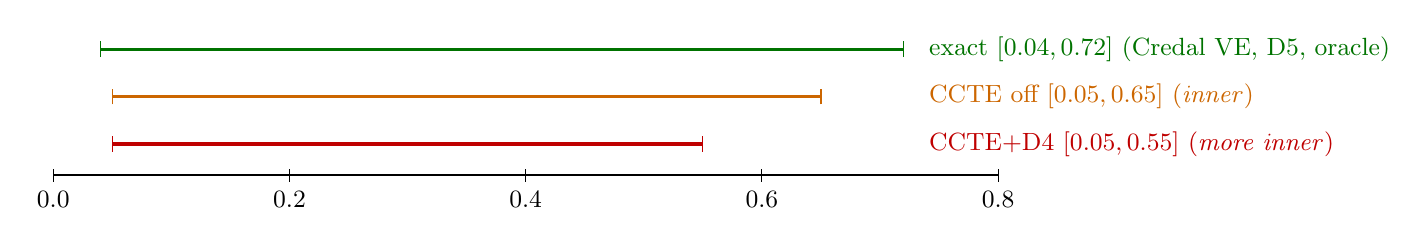
\begin{tikzpicture}[font=\small,>=Latex]
  \draw[thick] (0,0) -- (12,0);
  \foreach \x/\l in {0/0.0,3/0.2,6/0.4,9/0.6,12/0.8} \draw (\x,0.08)--(\x,-0.08) node[below]{$\l$};
  % exact
  \draw[very thick,green!45!black] (0.6,1.6) -- (10.8,1.6);
  \draw[green!45!black] (0.6,1.5)--(0.6,1.7); \draw[green!45!black] (10.8,1.5)--(10.8,1.7);
  \node[right,green!45!black] at (11.0,1.6) {exact $[0.04,0.72]$ (Credal~VE, D5, oracle)};
  % ccte off
  \draw[very thick,orange!80!black] (0.75,1.0) -- (9.75,1.0);
  \draw[orange!80!black] (0.75,0.9)--(0.75,1.1); \draw[orange!80!black] (9.75,0.9)--(9.75,1.1);
  \node[right,orange!80!black] at (11.0,1.0) {CCTE off $[0.05,0.65]$ (\emph{inner})};
  % ccte d4
  \draw[very thick,red!75!black] (0.75,0.4) -- (8.25,0.4);
  \draw[red!75!black] (0.75,0.3)--(0.75,0.5); \draw[red!75!black] (8.25,0.3)--(8.25,0.5);
  \node[right,red!75!black] at (11.0,0.4) {CCTE${+}$D4 $[0.05,0.55]$ (\emph{more inner})};
\end{tikzpicture}
\caption{$P(B)$ on \texttt{d4\_biting}. The exact strong-extension interval (green) is
  recovered by single-query Credal~VE and by \texttt{CredalJT}. CCTE's shared two-pass schedule
  (orange) lands strictly inside it, and the D4 filter (red) pushes further inward. CCTE is
  neither exact nor a valid outer bound once a cross-family sentence couples the families.}
\label{fig:dband}
\end{figure}

\subsection{Why the shared schedule, not D4, is the root cause}
It would be tempting to blame D4, but the \texttt{coupling="off"} row already fails: the inner
error is present before any filtering. The mechanism is dominance pruning at the wrong scope.
Single-query Credal~VE avoids it by giving each query its own order (query last); CCTE trades
that for a single all-marginals pass and therefore prunes on intermediate scopes shared by all
queries. On a cross-family-sentence-free instance this is harmless (Proposition~\ref{prop:exact};
the $3$-atom chain matches Credal~VE), because the surviving dominant function also dominates for
every downstream read-off. A cross-family sentence destroys that alignment: the function carrying
the extremal $P(B)$ is dominated \emph{in the marginalized bucket} yet is the unique maximizer of
the final $P(B)$, so pruning discards it. This is intrinsic to sharing one schedule across all
marginals; it is exactly why CCTE declines to augment the order (which would fix $P(B)$ but
loosen other atoms) and why D5/\texttt{CredalJT}, which never prunes vertices, is the correct
engine when a cross-family sentence is present.

\section{Verdict}\label{sec:verdict}

\begin{proposition}[What the experiments establish for CCTE]\label{prop:verdict}
For the marginal task on binary chain-graph LCNs:
\begin{enumerate}
  \item[\textnormal{(i)}] \textbf{CCTE bounds the strong extension} $\DSE\supseteq\DLCN$
    (Prop.~\ref{prop:target}), inheriting both looseness gaps A and B from the shared credal
    network.
  \item[\textnormal{(ii)}] \textbf{D1, D2, D3 tighten CCTE for free} at build time (no CCTE code
    change --- it reads narrower vertices); D1 measurably tightens \texttt{alarm}'s $P(A)$ from
    $[0.000,0.618]$ to $[0.014,0.606]$. \textbf{D4 is built into CCTE}
    (\texttt{coupling="cross-family"}) as a prune-time filter. \textbf{D5 is a separate engine}
    (\texttt{CredalJT}), unreachable by CCTE and the only sound choice for conditional queries.
  \item[\textnormal{(iii)}] \textbf{CCTE is exact on a clean singly-connected,
    cross-family-sentence-free LCN} (Prop.~\ref{prop:exact}), where $\DSE=\DLCN$ and the shared
    schedule is lossless --- verified on a $3$-atom chain (CCTE $=$ Credal~VE $=$ exact).
  \item[\textnormal{(iv)}] \textbf{A cross-family \emph{sentence} breaks both exactness and
    outer-ness.} On \texttt{d4\_biting}, CCTE \texttt{off} returns $P(B)=[0.05,0.65]$ ---
    strictly \emph{inside} the exact $[0.04,0.72]$ that Credal~VE, \texttt{CredalJT}, and two
    oracles all report --- and D4 pushes it further to $[0.05,0.55]$. The cause is dominance
    pruning on the single shared elimination order, not the D4 filter.
\end{enumerate}
\end{proposition}

\paragraph{Practical takeaway.} Use CCTE when you need \emph{all} marginals cheaply on a
cross-family-sentence-free chain graph, and take advantage of the free D1/D2/D3 build-stage
tightening (and $\varepsilon$-pruning to keep the function sets bounded). The moment the LCN
contains a cross-family sentence --- the same condition under which the strong extension departs
from $\DLCN$ --- CCTE is neither exact nor a guaranteed outer bound: prefer single-query
Credal~VE for one unconditional marginal, and \texttt{CredalJT} (D5) for exact all-marginals or
any conditional query.

\paragraph{Reproducibility.} All numbers come from \texttt{examples/d4\_biting.lcn}
(3 atoms), a clean $3$-atom Markov chain, and \texttt{examples/alarm.lcn}, run through
\texttt{CredalNetworkVertices.from\_lcn} (\texttt{method="linear"} / \texttt{"linear-tight"})
and \texttt{CredalCTE.run} (\texttt{coupling="off"} / \texttt{"cross-family"}). The exact
references are single-query \texttt{CredalVE.run}, \texttt{CredalJT.run(solver="scip")}, a
parametric SLSQP oracle satisfying $(B\indep C\mid A)$ by construction, and a strong-extension
vertex-enumeration oracle.

\end{document}
